\chapter{Methodology}
\label{chap:methodology}


\section{Dataset}
\label{sec:dataset_description}

I used a collection of radar images to train and evaluate the models. These radar images were composites from a heterogeneous network of operational weather radars created by \gls{OPERA} \cite{weatherradar}. In October 2013, the network consisted of 202 operational radars, of which 184 had Doppler capability and 48 were dual-polarization radars. Most radars operate at the C band (168 sites). However, several S-band radars are installed in the south of Europe (33 sites)\footnote{For more information about different radars used in weather nowcasting, refer to section \ref{subsec:radars}}.

\begin{figure}[ht]
    \centering
    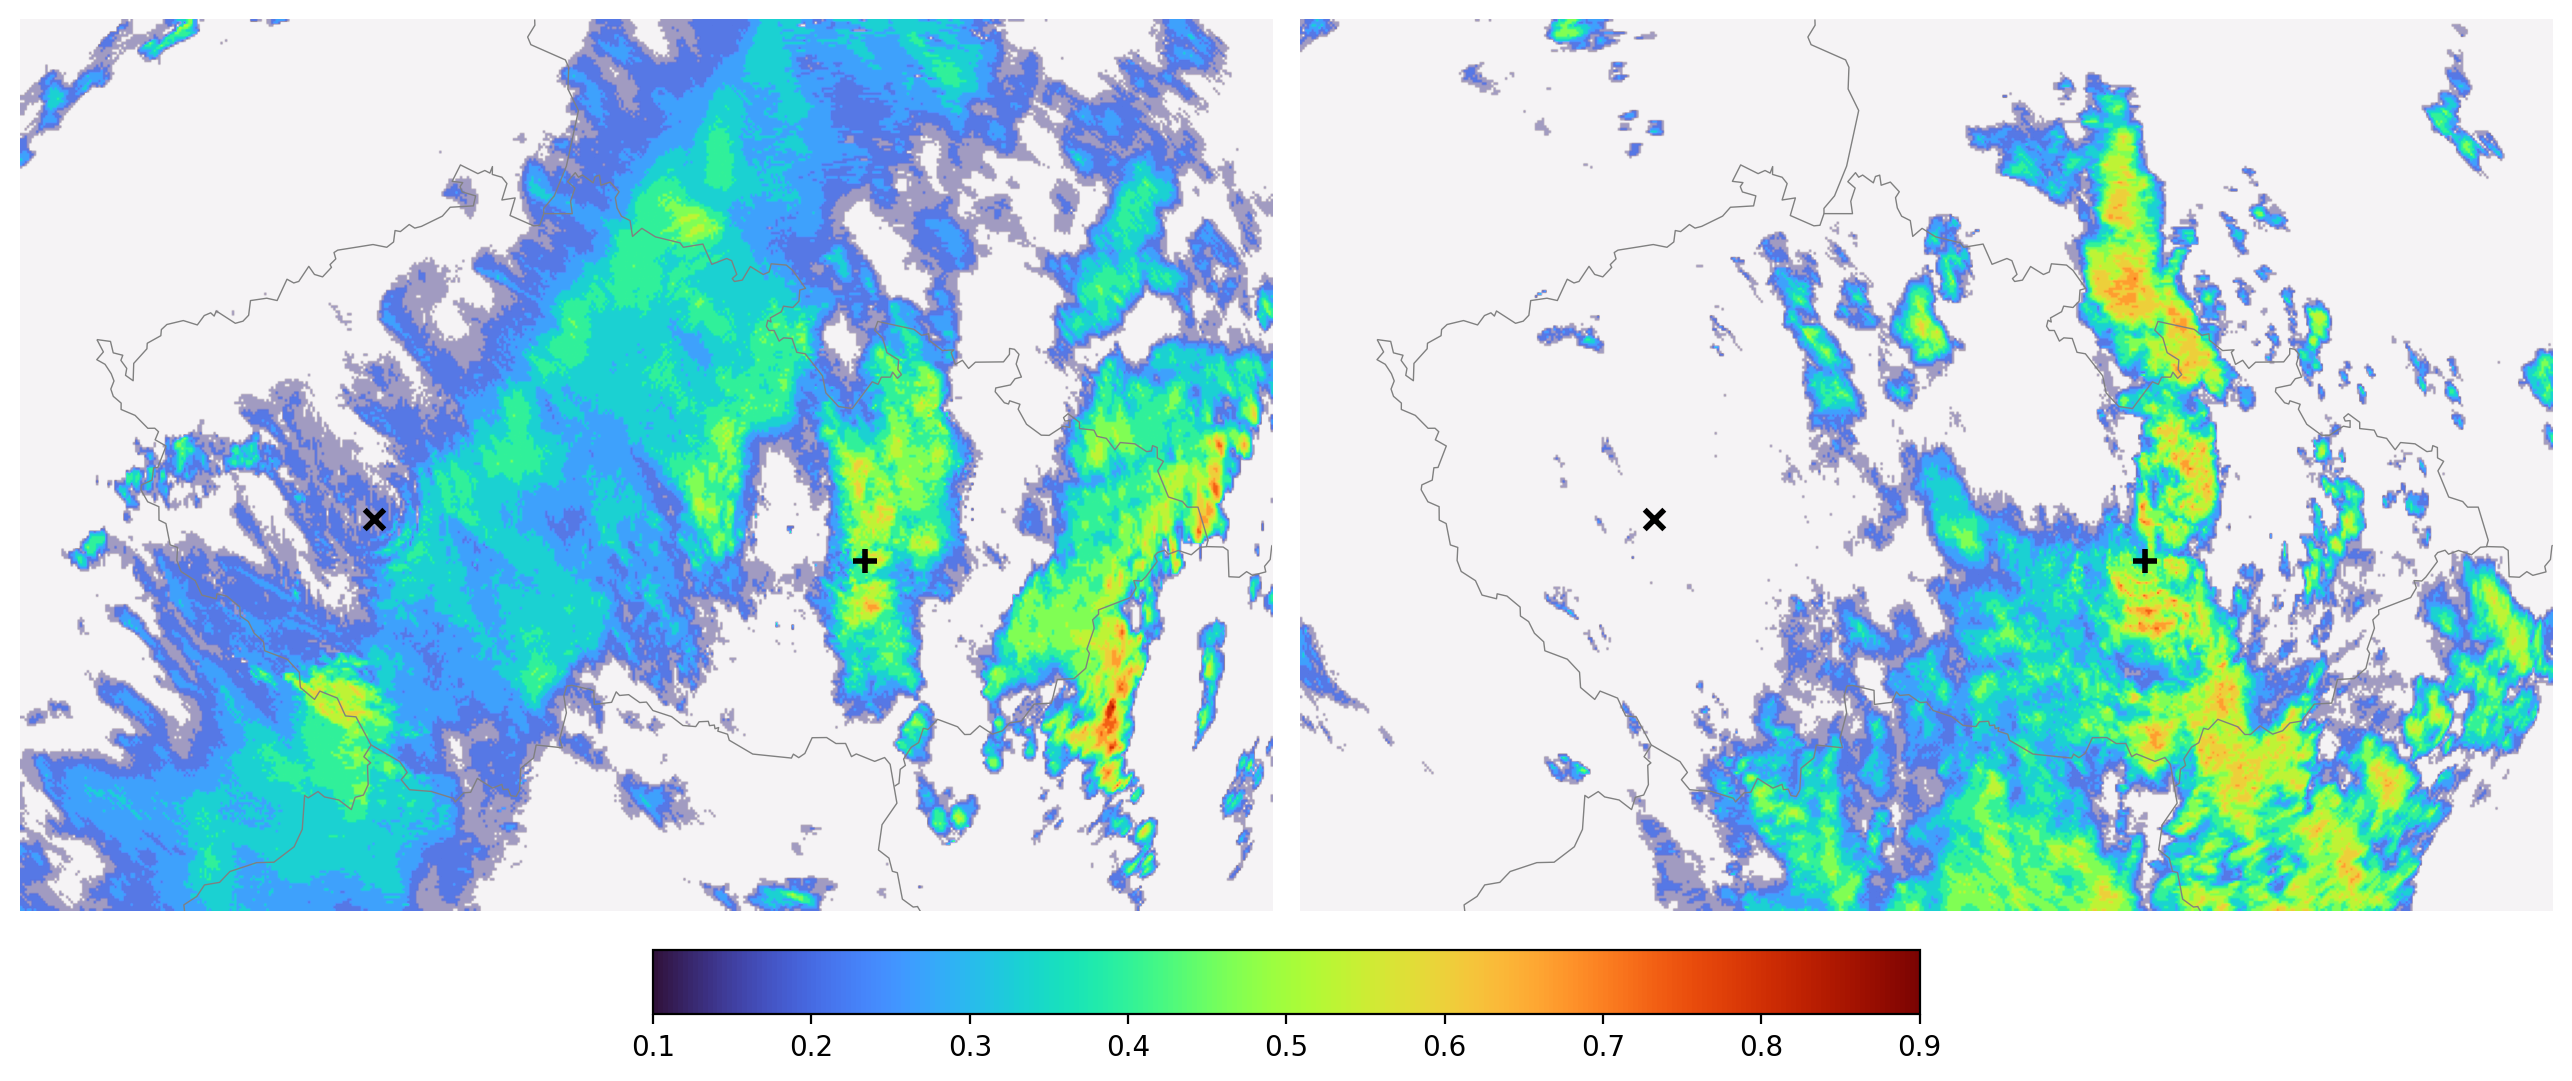
\includegraphics[width=\textwidth]{images/radar_image_with_map.png}
    \caption[Example of radar images from the dataset]{\label{fig:radar_image_with_map}Example of images from the dataset after preprocessing. Values smaller than the lower bound of the color bar are transparent, and those higher than the upper bound are displayed as if they were equal to it. Positions of Czech radars are marked with symbols × (Brdy-Praha) and + (Skalky).}
\end{figure}

The \gls{OPERA} Radar Data Center (Odyssey) has been operational since 2011. Polar volume data are collected from 134 radar sites in 21 countries, and continental scale mosaic products (surface rain rate, rainfall accumulation, and maximum reflectivity) are generated in real-time. These mosaic products are generated on a Cartesian grid covering Europe (3800×4400 $\text{km}^2$). \cite{weatherradar}

The images I used cover the area above the Czech Republic, as illustrated in figure \ref{fig:radar_image_with_map}. The resolution of images is 544×352 pixels, where one pixel represents an area of 1 $\text{km}^2$. Images are generated every 10 minutes, but some may be missing. Absent images were taken into account when creating network inputs and targets. The dataset covers the period from October 23, 2015, to July 21, 2020.

\subsection{Data Preprocessing and Augmentation}
\label{sec:data_preprocessing}

The radar data from \gls{OPERA} was already cleaned using a combination of anomaly removal and hit-accumulation clutter filtering, which was done by the anomaly-removal module\footnote{Some anomalies are still visible in the figure \ref{fig:radar_image_with_map} in the form of circles around the radars.}.

In the mosaic, each pixel comprises of data from different multiple radars and elevations. The highest value from all the available heights and radars is chosen for each pixel. The dataset's images have a maximum reflectivity captured in 16 values ranging from 0 to 60 dBZ. These values are then mapped to a range of 0 to 255. I utilized min-max normalization to ensure all values ranged from 0 to 1. I then cropped a rectangle of 512×256 pixels from the images, preventing pooling problems\footnote{Pooling is used in both models with 2×2 stride and 2×2 kernel, which halves the feature resolution in both axes. This pooling can be performed without padding or dropping values when the images have sides equal to powers of two. See section \ref{subsec:convolution} about convolution and section \ref{subsec:pooling} about pooling.}.

\begin{figure}[ht]
    \centering
    \begin{subcaptionblock}[t]{.45\textwidth}
        \centering
        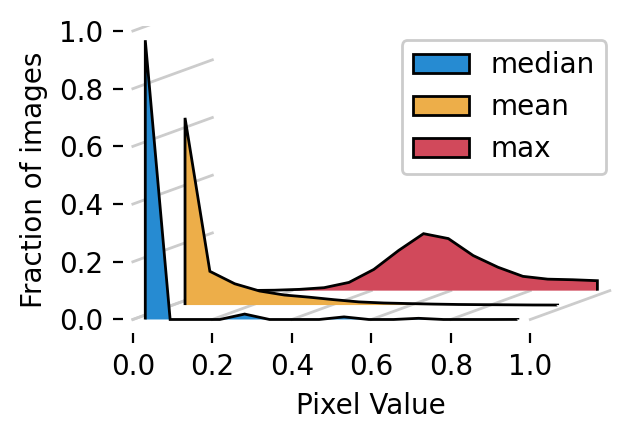
\includegraphics[width=\textwidth]{images/hist_dataset.png}
        \caption[Distribution maximum, median, and mean values for each image in the dataset]{\label{fig:hist_dataset}Distribution of maximum, median, and mean values for each image in the dataset.}
    \end{subcaptionblock}
    \hspace{1em}
    \begin{subcaptionblock}[t]{.45\textwidth}
        \centering
        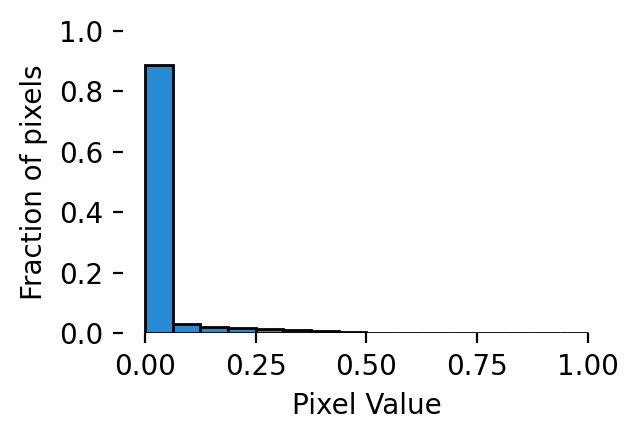
\includegraphics[width=\textwidth]{images/hist_dataset_pixels.png}
        \caption[Distribution of pixel values in the dataset]{Distribution of individual pixel values in the dataset.}
    \end{subcaptionblock}
    \caption[Distribution of radar echo intensities in the dataset]{Distribution of radar echo intensities in the dataset.}
\end{figure}

I did not exclude any images from the data. In hindsight, it may have been a mistake not to do this because the dataset includes numerous almost empty images, as illustrated in figure \ref{fig:hist_dataset}.

\subsection{Creating Data Points}
\label{sec:data_points}

Both models were trained on a sequence of consecutive images spaced by parameter \texttt{stride}\footnote{Parameter \texttt{stride} is in minutes.}. The dataset was split into chunks, each containing \texttt{chunk\_size} of images from the sequence. Data points were generated by setting an \texttt{input\_length}, and \texttt{target\_length}.

A sliding window of length $\texttt{input\_length} + \texttt{target\_length}$ is then moved along the images in one chunk. Each position of the sliding window represents one data point for the models. The corresponding data point will not be created if the dataset has a missing image in data points inputs or outputs.

The dataset is split by randomly assigning generated chunks to some of the datasets. Two consecutive chunks have no overlap, which is essential for creating training, validation, and testing datasets. The probability of assigning a chunk to one of the datasets is given by parameters \texttt{test\_frac} and \texttt{val\_frac} representing fractions of the dataset which will be used for testing and validation respectively\footnote{The probability that these datasets will contain the same number of images is small, because, aside from the randomness, the chunks do not contain the same number of data points due to the missing images.}. Data points in assigning chunks are then concatenated to create the datasets. The random assigning can be seeded by setting the \texttt{seed} parameter. This way, the same datasets are generated each time.

\begin{figure}[ht]
    \centering
    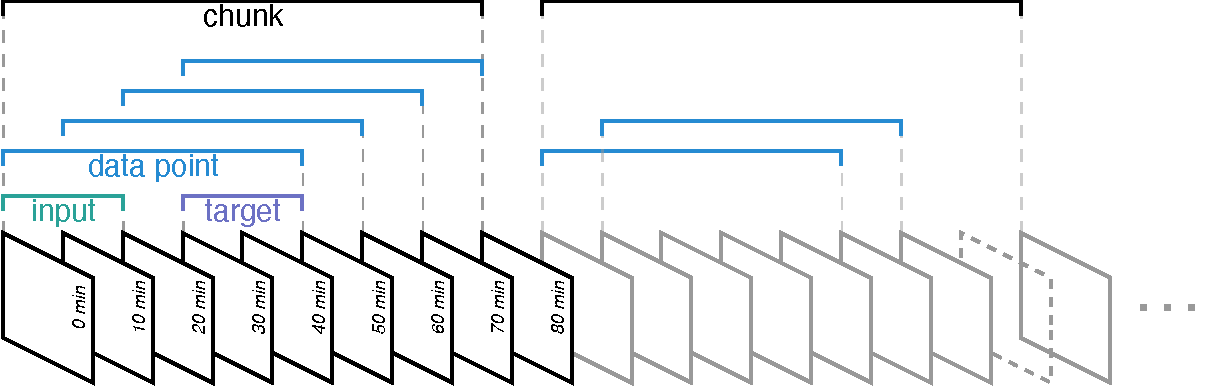
\includegraphics[width=\textwidth]{images/dataset.pdf}
    \caption[Process of generating data points from the dataset]{\label{fig:data_points}Generating data points from the dataset in chunks. Datapoint is added to the chunk only if it has no missing images in the input or target images. There is no overlap of data points between different chunks.}
\end{figure}

Adjusting the \texttt{chunk\_size}\footnote{Parameter \texttt{chunk\_size} needs to be $\geq$ than $\texttt{input\_length} + \texttt{target\_length}$.} changes the number of data points overall as smaller chunks skip more images to maintain no overlap between the chunks. I chose these values for the parameters:

\begin{align*}
    &\texttt{stride} = 10,&  &\texttt{test\_frac} = 0.1,& &\texttt{val\_frac} = 0.1,& &\texttt{seed} = 42, \\
    &\texttt{chunk\_size} = 100,& &\texttt{input\_length} = 8,& &\texttt{target\_length} = 8.&    &
\end{align*}

\noindent This resulted in training, validation, and testing datasets with 168110, 21108, and 20957 data points, respectively. The whole process is depicted in figure \ref{fig:data_points}.

\section{UNet}
\label{sec:standard_unet}

I chose similar architecture as in the original paper \cite{unet}. The network has five ``levels'', meaning five pooling and transposed convolution layers exist. The encoder layer consists of a convolution block and max pooling. As mentioned earlier, max pooling is done with 2×2 strides and 2×2 kernel.

Convolution block is a sequence of 2D convolution followed by Batch normalization, ReLU, and Dropout. The convolution block can be repeated multiple times. I chose to do three repetitions. All 2D convolutions in the block are executed with 1×1 stride and 3×3 kernel and 1×1 padding\footnote{In practice, it would be better to use no padding and therefore have smaller output than input. Doing it this way guarantees the same network output near edges when tiling larger surfaces. See \cite[fig. 2]{unet}}.

\textit{Batch normalization} is a technique used in deep learning to improve the training process of artificial neural networks\footnote{See paper \cite{batchnorm}.}. I used it as it has been shown to improve training speed, enable the use of higher learning rates, and often lead to better generalization performance. \textit{Dropout} is a regularization technique used in neural networks to prevent overfitting and improve generalization\footnote{See paper \cite{dropout}}. During the training process, Dropout randomly ``drops out"\footnote{I. e. temporarily removes or sets to 0.} a proportion of the neurons in a given layer at each training step. The dropped-out neurons do not contribute to that training iteration's forward or backward pass. A hyperparameter called the \texttt{dropout\_rate} can set the probability of a neuron being dropped.

The number of output channels from the convolution block can be adjusted by setting different values of parameters \texttt{in\_channels} and \texttt{out\_channels}. The first convolution in the block changes the number of feature maps as described in the section \ref{subsec:convolution} and figure \ref{fig:convolution_kernel_collection}. In the encoder, the number of features is doubled each time.

The decoder layer begins with a transposed convolution. The output of this operation is then combined with a feature from the skip connection. Convolution block follows, but this time the number of features is halved. The transposed convolution also halves the number of features. It has a 2×2 stride and variable kernel size, which is given by parameter \texttt{kernel\_size} when the network is initialized. I will examine how this parameter's best value was found later in the section \ref{subsec:hyperparameters}. Padding in transposed convolution must be adjusted based on the kernel size to $\lfloor (k - 2) / 2 \rfloor$.

Finally, preventing some artifacts which may appear from the transposed convolution is achieved by 2D convolution with 1×1 stride and 1×1 kernel. Moreover, I added a sigmoid activation as the network's last layer to make the network outputs in the correct range. Figure \ref{fig:my_unet_diagram} shows a diagram of the implementation. The network used for eventual training had 11 713 080 parameters, all trainable. The size of the weights is 44.68 MB.

\begin{figure}[ht]
    \centering
    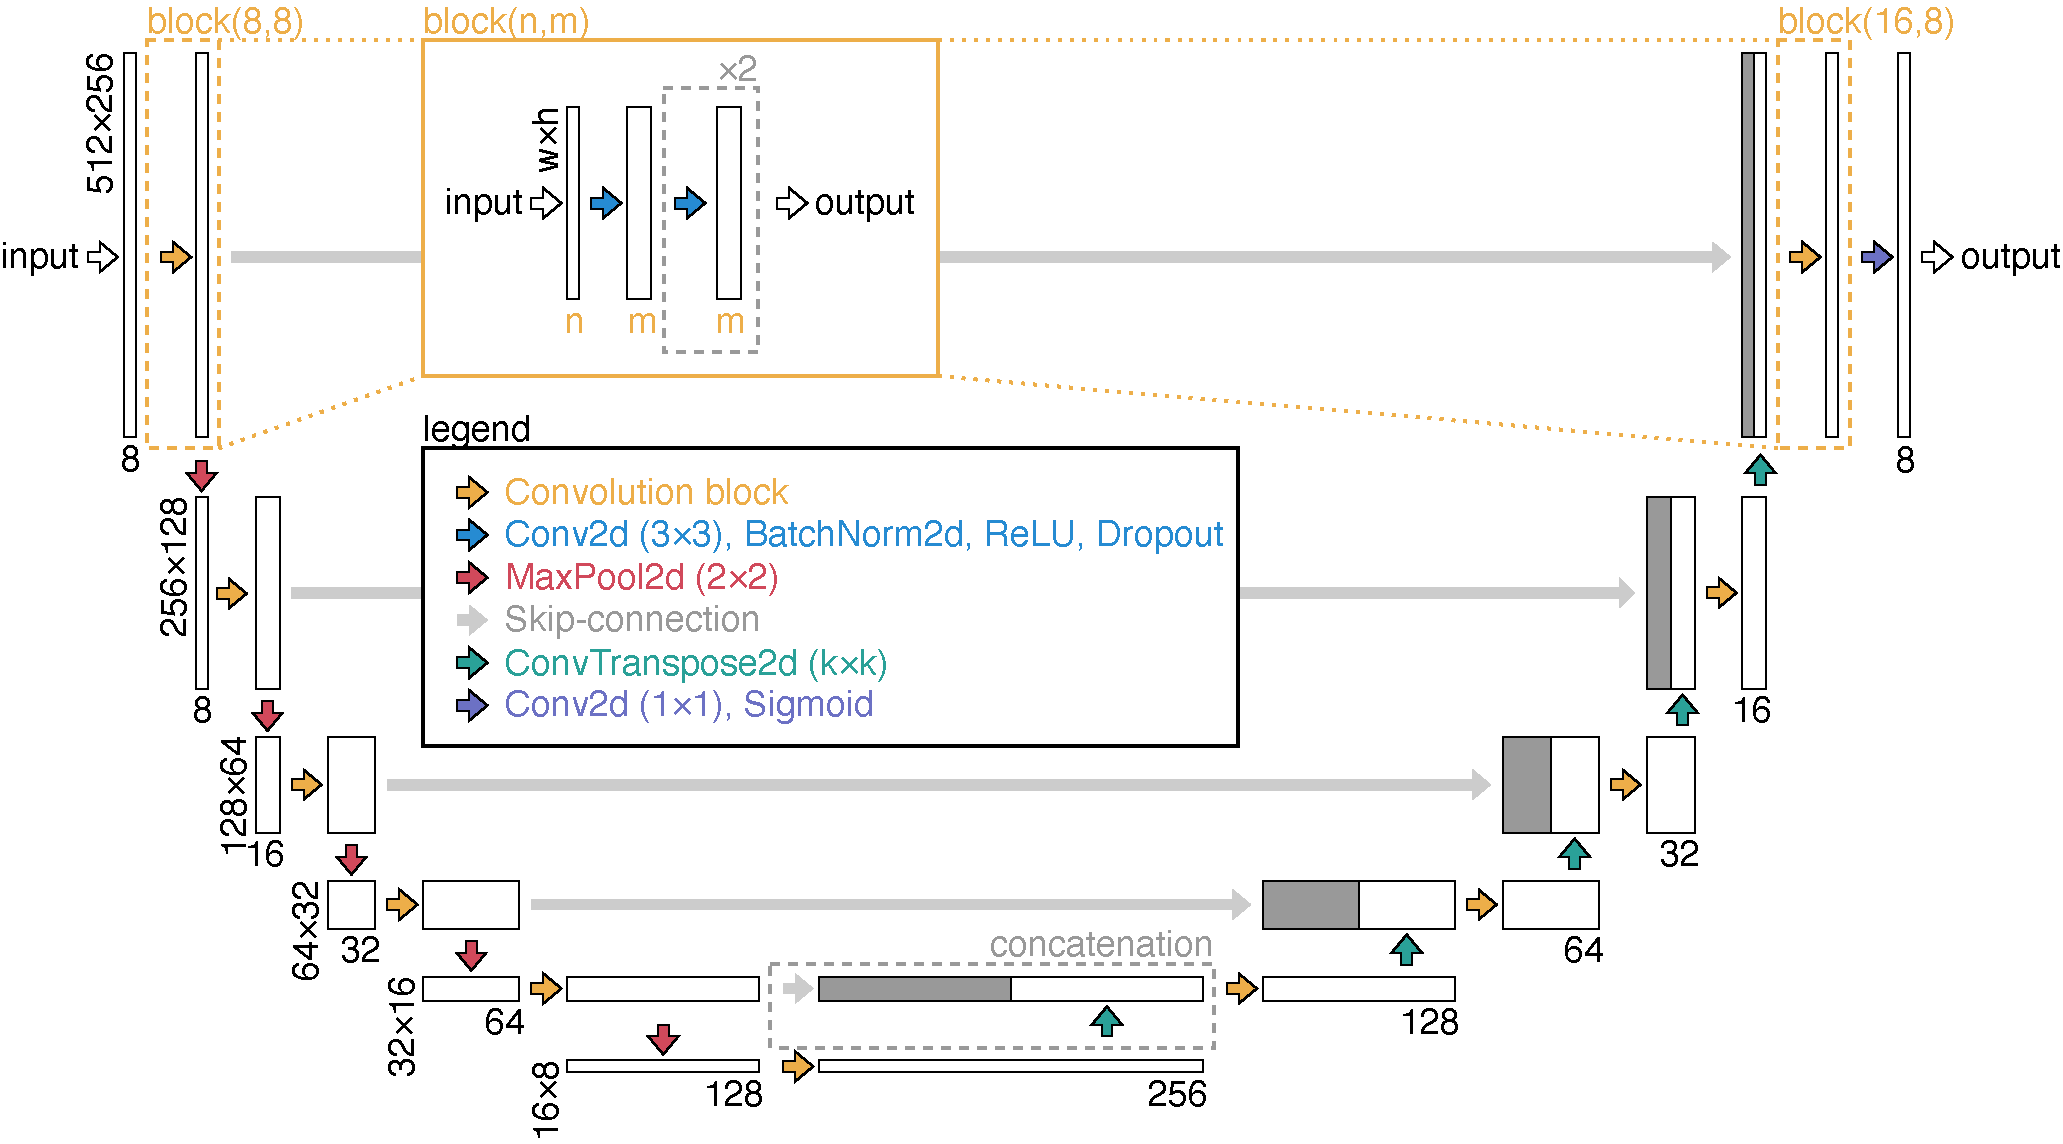
\includegraphics[width=\textwidth]{images/my_unet_diagram.pdf}
    \caption[UNet implementation diagram]{\label{fig:my_unet_diagram}UNet implementation diagram.}
\end{figure}

\section{GUNet}
\label{sec:methodology_gunet}

My implementation of the \gls{GUNet} architecture is inspired by the one in the paper \cite{gunet}. It is similar to the UNet, as portrayed in figure \ref{fig:my_gunet_diagram}. The convolution block, which follows the same structure as in the UNet architecture, uses 1×1 stride, 3×3 kernel, and 1×1 padding for all 2D convolutions. The network's final layers utilize 2D convolution with a 1×1 stride and 1×1 kernel, along with sigmoid activation.

Upsampling modules inside the decoder are replaced by \gls{GU}\footnote{Workings of \gls{GU} are described in section \ref{subsec:guided_upsampling}}. The \gls{GIF} in \gls{GU} has two parameters\footnote{See section \ref{subsec:guided_image_filtering}}: $\epsilon$, a regularization parameter penalizing large $a_k$ and $r$ which is a radius defining $\omega_{k}$. The value of these parameters was found by hyperparameter search, which I explore in the section \ref{subsec:hyperparameters}. Using \gls{GIF} instead of transposed convolution lowered the number of trainable parameters to 10 578 728, which take up 40.35 MB.

\begin{figure}[ht]
    \centering
    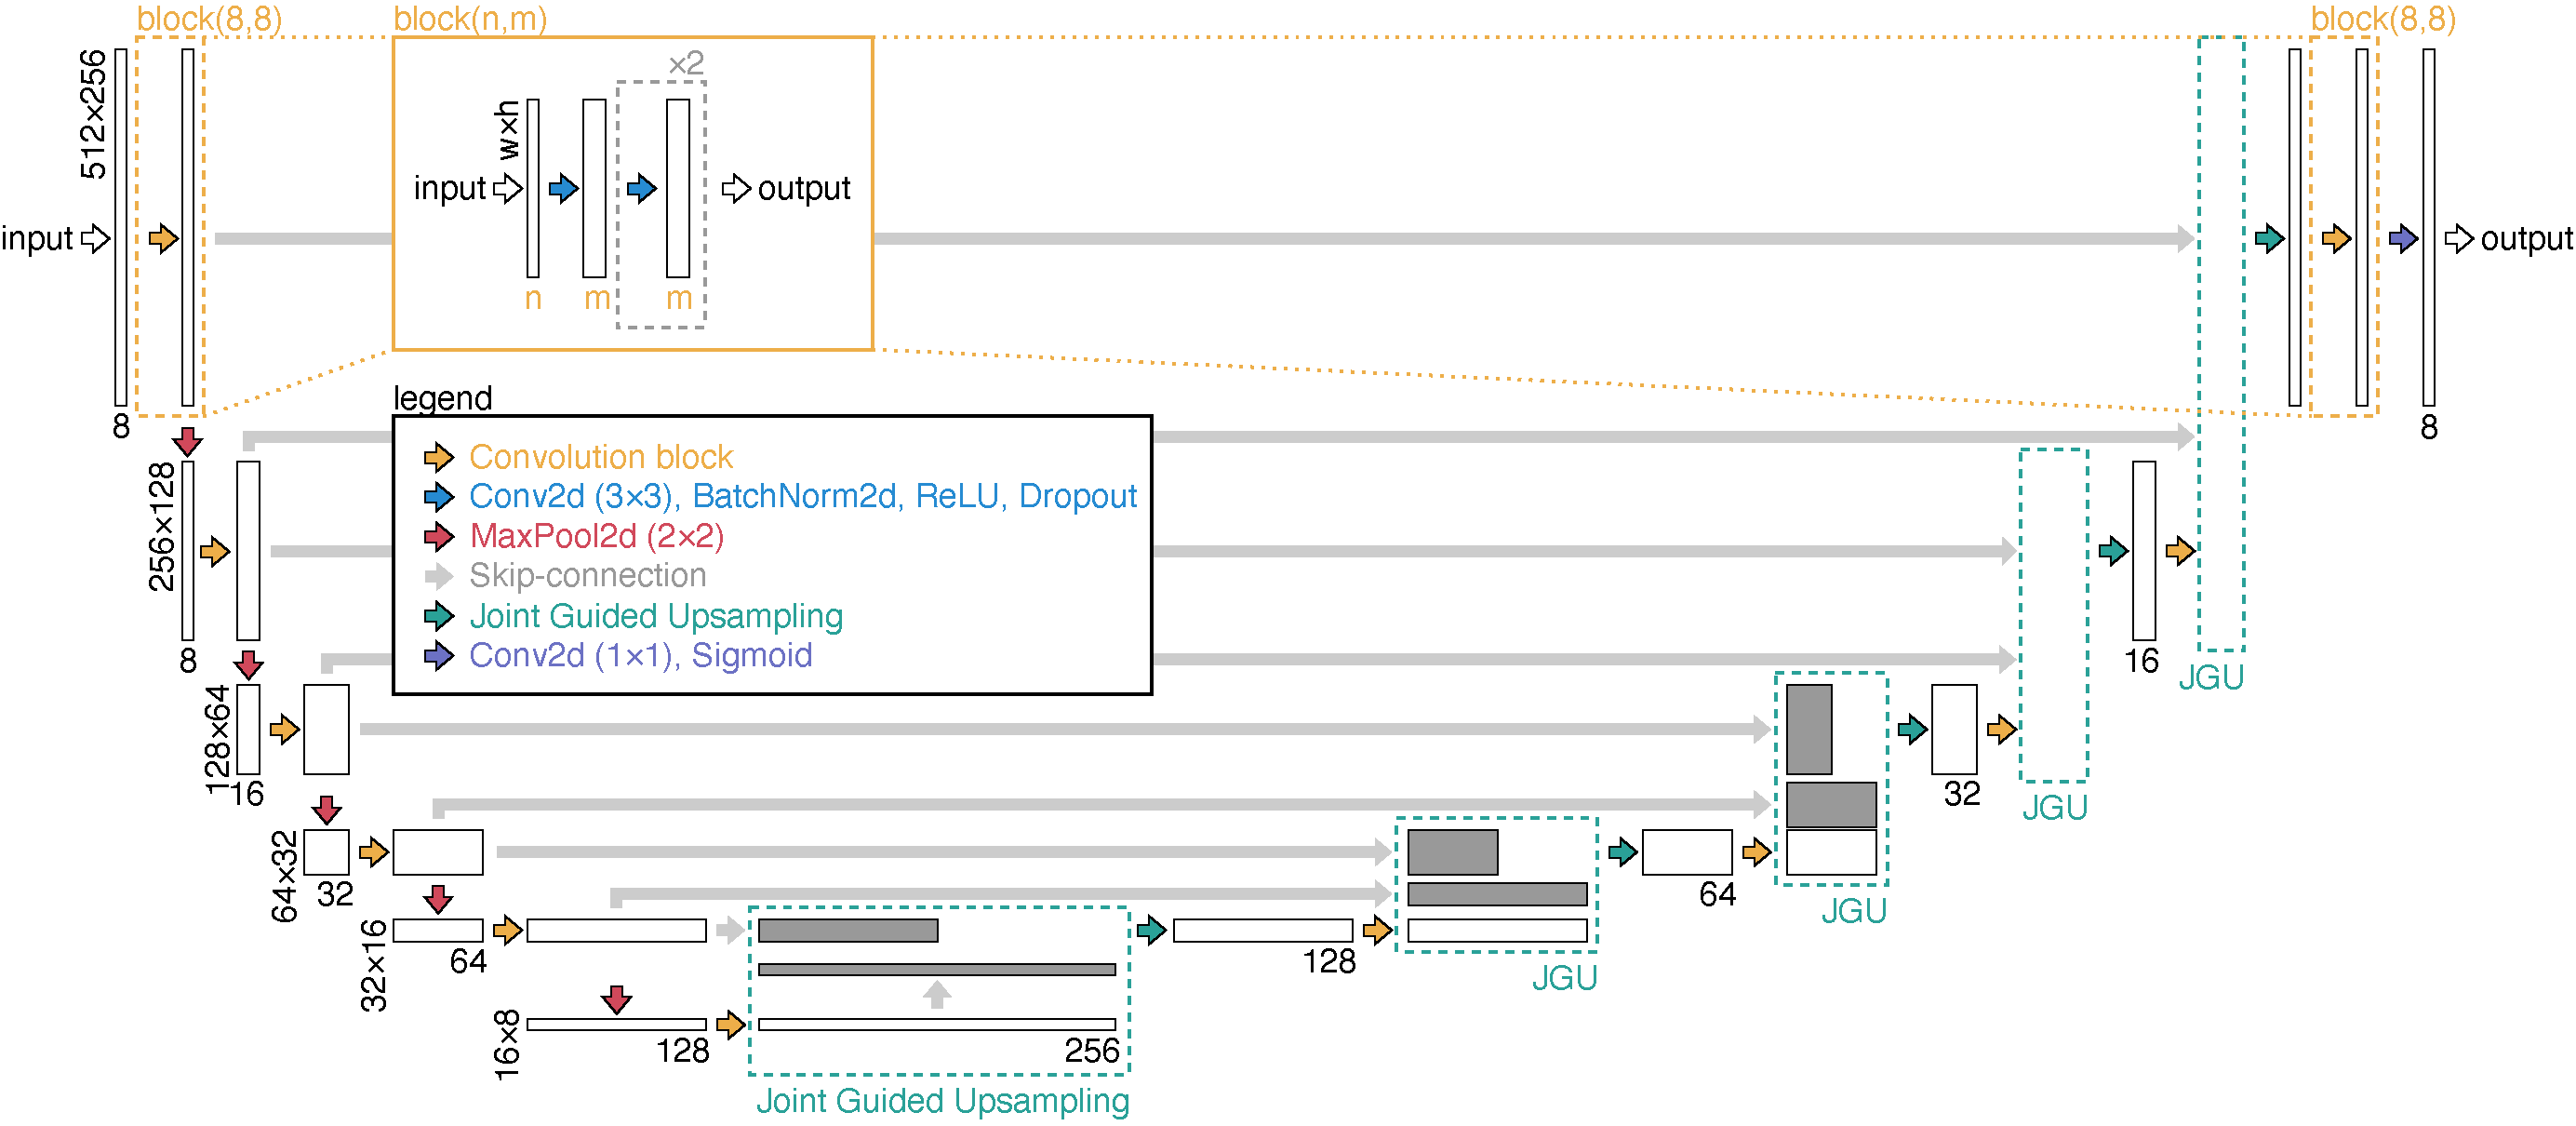
\includegraphics[width=\textwidth]{images/my_gunet_diagram.pdf}
    \caption[GUNet implementation diagram]{\label{fig:my_gunet_diagram}GUNet implementation diagram.}
\end{figure}

\subsection{Feature Channel Count Discrepancy}
\label{subsed:channel_discrepancy}

The \gls{GU} was implemented by slightly adjusting the \gls{GIF} implementation from the paper \cite{fastguidedtrainable}. In the paper \cite{gunet}, the authors mention that the \gls{GIF} should be applied on each channel separately. Here I ran into an issue because, as shown in figure \ref{fig:my_gunet_diagram} and discussed previously in the section \ref{subsec:review_gunet_architecture},  the \gls{GUNet} architecture's lower layers have more channels than the higher ones.

The issue with the feature channels in the "higher" and "lower" skip-connections is that the number of channels in the feature from the "higher" skip-connection used as the higher resolution guide, $I^\texttt{hr}$, is not the same as the number of channels in the feature from the "lower" skip-connection used as the lower resolution guide, $I^\texttt{lr}$. The filter, therefore, cannot be applied on each channel separately, as implied in the paper \cite{gunet}.

I contacted the authors of this paper about this issue and learned that they used an identical channel count on each ``level'' of their networks, which seemed odd because the diagram in \cite[fig. 2]{gunet} displayed higher channel counts in the "lower" layers of the UNet. After further consultation with my advisor, I decided to reduce the number of channels in the coefficients $\bar a_k^{\texttt{hr}}$ and $\bar b_k^{\texttt{hr}}$, using 2D convolution with 1×1 stride and 1×1 kernel. The coefficients then can be utilized with the higher resolution guidance feature $I^{\texttt{hr}}$ to compute the final filtered decoder feature with equation \ref{eq:guided_upsampling}.

\section{Model Optimization}

Both networks were implemented in PyTorch and trained on the NVIDIA A100-SXM4-40GB graphics card.

\subsection{Hyperparameter Tuning}
\label{subsec:hyperparameters}

For finding values of tunable hyperparameters of both networks, I used a hyperparameter optimization framework called Optuna, from paper \cite{optuna}. I used the default \gls{TPE} algorithm\footnote{To learn more about the TPE algorithm, please refer to the paper cited as \cite[pg. 4]{tpe}.}. I created a study of 50 trials for each model. Each trial could have run for at most five epochs, where one epoch passed over all data points in the training dataset. Batch sizes for both models were set to 70. I used the Adam optimizer \cite{adam}. Trials were compared based on average \gls{SSIM}\footnote{See the section \ref{subsec:val_metrics}.} value on the whole validation dataset. Based on this validation metric, trials could be pruned sooner than after five epochs. The parameters from the trial with the highest \gls{SSIM} score were selected after conducting 50 trials. These parameters were then used for training the networks. The search space for the UNet consisted of parameters:
\begin{align*}
    &\texttt{learning\_rate} \in [10^{-5},10^{-1}],     &   &\texttt{dropout\_rate} \in [10^{-5},0.5],\\
    &\texttt{loss} \in \{\texttt{mse},\texttt{mae}\},   &   &\texttt{kernel\_size} \in \{2,4,6,8\}.
\end{align*}

\noindent Odd sizes of kernels were skipped because of artifacts mentioned in the section \ref{subsec:structural_bias}, created when the kernel size is not divisible by the stride, which is 2×2 in the case of transposed convolution in the UNet. The best values from the search were:
\begin{align*}
    &\texttt{learning\_rate} \approx 0.0100,  &   &\texttt{dropout\_rate} \approx 0.0160, & &\texttt{loss} = \texttt{mse},\\
    &\texttt{kernel\_size} = 2.
\end{align*}

\noindent The search space for the \gls{GUNet} consisted of parameters:
\begin{align*}
    &\texttt{learning\_rate} \in [10^{-5},10^{-1}],     &   &\texttt{dropout\_rate} \in [10^{-5},0.5],\\
    &\texttt{loss} \in \{\texttt{mse},\texttt{mae}\},   &   &\texttt{epsilon} \in [10^{-5},1], \\
    &\texttt{radius} \in \{1,2,3\}.
\end{align*}

\noindent The best values from the search were:
\begin{align*}
    &\texttt{learning\_rate} \approx 0.0031,    &   &\texttt{dropout\_rate} \approx 0.0024,&  &\texttt{loss} = \texttt{mse},\\
    &\texttt{epsilon} \approx 0.1483,           &   &\texttt{radius} = 2.
\end{align*}

\subsection{Training}
\label{subsec:training}

Both models were trained with the parameters found in the search for 100 epochs, again with the Adam optimizer. During training, I measured the progress with \gls{SSIM}, \gls{MAE}, and \gls{MSE}. When computing these metrics, I have set the models to evaluation mode. When the models are in this mode, particular layers like Dropout and BatchNorm will behave differently to ensure the network produces deterministic outputs. In this mode, dropout layers will not drop any activations, and batch normalization layers will use the running mean and variance calculated during training rather than the statistics of the current batch.

The best values in these metrics measured on the validation dataset for the UNet were:

\begin{align*}
    &\texttt{\gls{SSIM}}: 0.8713, & &\texttt{\gls{MAE}}: 0.01269, & &\texttt{\gls{MSE}}: 0.0019390
\end{align*}

\noindent and the best values for the GUNet were:

\begin{align*}
    &\texttt{\gls{SSIM}}: 0.8693, & &\texttt{\gls{MAE}}: 0.01290, & &\texttt{\gls{MSE}}:0.0019398.
\end{align*}

Progress of the training is captured in figure \ref{fig:training}. Both networks' capabilities are comparable, although UNet performed slightly better in all metricsThe UNet was trained in a shorter amount of time, as shown in figure \ref{fig:val_ssim_duration}\footnote{The model architecture may not have affected this as the training was not the only process running on the GPUs}.


\begin{figure}[ht]
    \centering
    \begin{subcaptionblock}[t]{0.49\textwidth}
        \centering
        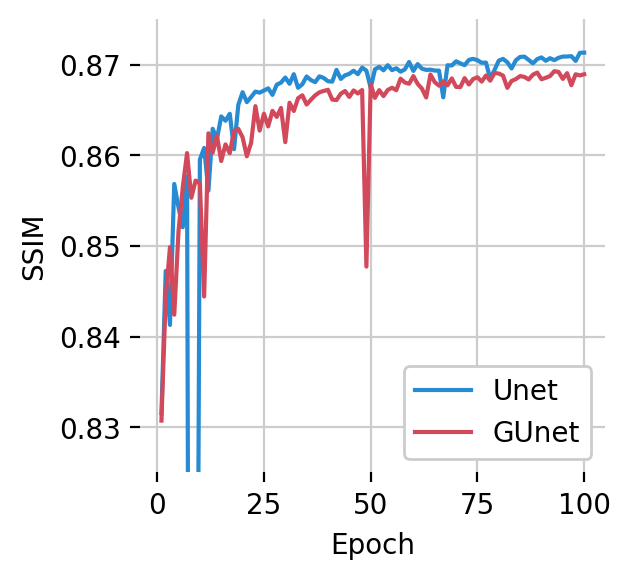
\includegraphics[width=\textwidth]{images/val_ssim_epoch.png}
        \caption{\label{fig:val_ssim_epoch}}
    \end{subcaptionblock}
    \begin{subcaptionblock}[t]{0.49\textwidth}
        \centering
        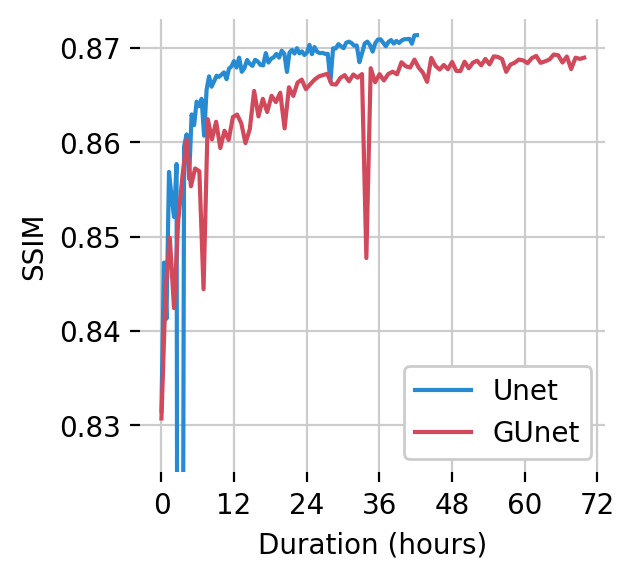
\includegraphics[width=\textwidth]{images/val_ssim_duration.png}
        \caption{\label{fig:val_ssim_duration}}
    \end{subcaptionblock}
    \begin{subcaptionblock}[t]{0.49\textwidth}
        \centering
        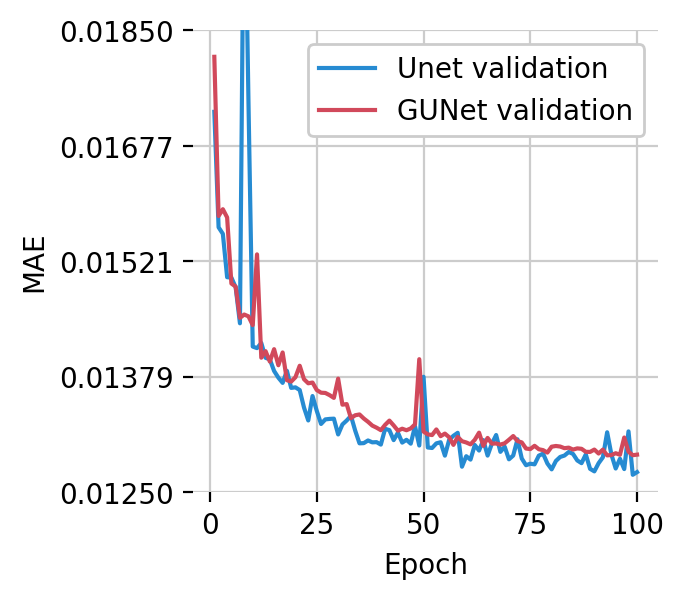
\includegraphics[width=\textwidth]{images/val_mae_epoch.png}
        \caption{\label{fig:val_mae_epoch}}
    \end{subcaptionblock}
    \begin{subcaptionblock}[t]{0.49\textwidth}
        \centering
        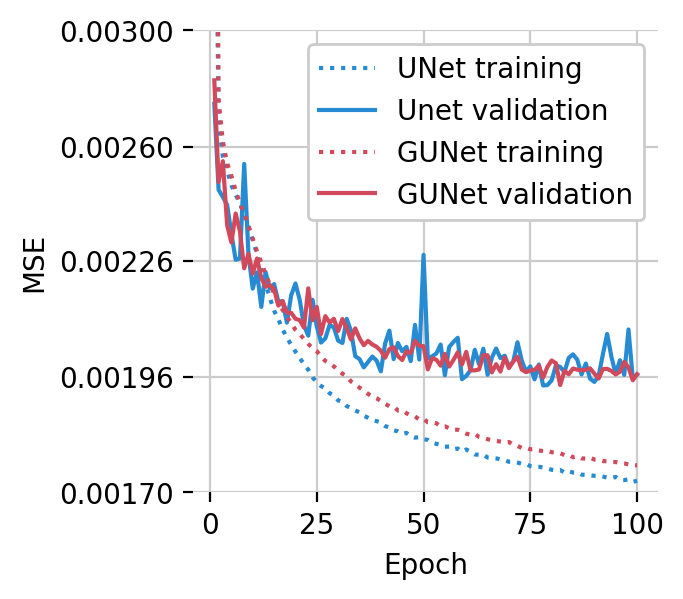
\includegraphics[width=\textwidth]{images/train_val_mse_epoch.png}
        \caption{\label{fig:train_val_mse_epoch}}
    \end{subcaptionblock}
    \captionsetup{subrefformat=parens}
    \caption[Training progress]{\label{fig:training}Training progress quantified by \gls{SSIM}, \gls{MAE} and \gls{MSE}. Relationship between \gls{SSIM} and the number of epochs can be seen in \subref{fig:val_ssim_epoch}, while \subref{fig:val_ssim_duration} shows \gls{SSIM} as a function of training time. \gls{MAE} on the validation dataset is in \subref{fig:val_mae_epoch}. \gls{MSE} was measured on the training data, too, as it was used as a loss function for training. Comparison between training and validation loss can be seen in \subref{fig:train_val_mse_epoch}.}
\end{figure}